\titledquestion{Understanding word2vec}[15]
Recall that the key insight behind {\tt word2vec} is that \textit{`a word is known by the company it keeps'}. Concretely, consider a `center' word $c$ surrounded before and after by a context of a certain length. We term words in this contextual window `outside words' ($O$). For example, in Figure~\ref{fig:word2vec}, the context window length is 2, the center word $c$ is `banking', and the outside words are `turning', `into', `crises', and `as':

\begin{figure}[h]
    \centering
    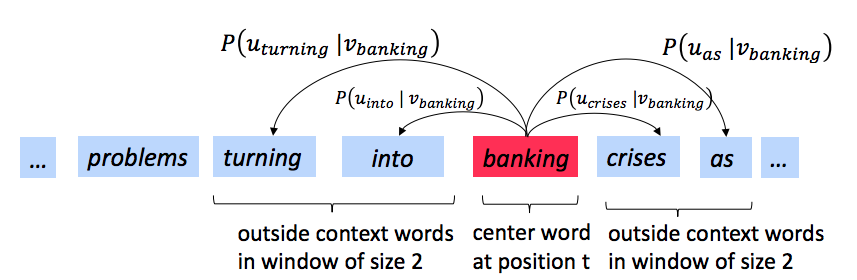
\includegraphics[width=0.6\textwidth]{word2vec.png}
    \caption{The word2vec skip-gram prediction model with window size 2}
    \label{fig:word2vec}
\end{figure}

Skip-gram {\tt word2vec} aims to learn the probability distribution $P(O|C)$. 
Specifically, given a specific word $o$ and a specific word $c$, we want to predict $P(O=o|C=c)$: the probability that word $o$ is an `outside' word for $c$ (i.e., that it falls within the contextual window of $c$).
We model this probability by taking the softmax function over a series of vector dot-products: % I added the word "softmax" here because I bet a lot of students will have forgotten what softmax is and why the loss fn is called naive softmax. but if this is too wordy we can just take it out

\begin{equation}
 P(O=o \mid C=c) = \frac{\exp(\bu_{o}^\top \bv_c)}{\sum_{w \in \text{Vocab}} \exp(\bu_{w}^\top \bv_c)}
 \label{word2vec_condprob}
\end{equation}

For each word, we learn vectors $u$ and $v$, where $\bu_o$ is the `outside' vector representing outside word $o$, and $\bv_c$ is the `center' vector representing center word $c$. 
We store these parameters in two matrices, $\bU$ and $\bV$.
The columns of $\bU$ are all the `outside' vectors $\bu_{w}$;
the columns of $\bV$ are all of the `center' vectors $\bv_{w}$. 
Both $\bU$ and $\bV$ contain a vector for every $w \in \text{Vocabulary}$.\footnote{Assume that every word in our vocabulary is matched to an integer number $k$. Bolded lowercase letters represent vectors. $\bu_{k}$ is both the $k^{th}$ column of $\bU$ and the `outside' word vector for the word indexed by $k$. $\bv_k$ is both the $k^{th}$ column of $\bV$ and the `center' word vector for the word indexed by $k$. \textbf{In order to simplify notation we shall interchangeably use $k$ to refer to word $k$ and the index of word $k$.}}\newline

%We can think of the probability distribution $P(O|C)$ as a prediction function that we can approximate via supervised learning. For any training example, we will have a single $o$ and $c$. We will then compute a value $P(O=o|C=c)$ and report the loss. 
Recall from lectures that, for a single pair of words $c$ and $o$, the loss is given by:

\begin{equation} 
\bJ_{\text{naive-softmax}}(\bv_c, o, \bU) = -\log P(O=o| C=c).
\label{naive-softmax}
\end{equation}

We can view this loss as the cross-entropy\footnote{The \textbf{cross-entropy loss} between the true (discrete) probability distribution $p$ and another distribution $q$ is $-\sum_i p_i \log(q_i)$.} between the true distribution $\by$ and the predicted distribution $\hat{\by}$, for a particular center word c and a particular outside word o. 
Here, both $\by$ and $\hat{\by}$ are vectors with length equal to the number of words in the vocabulary.
Furthermore, the $k^{th}$ entry in these vectors indicates the conditional probability of the $k^{th}$ word being an `outside word' for the given $c$. 
The true empirical distribution $\by$ is a one-hot vector with a 1 for the true outside word $o$, and 0 everywhere else, for this particular example of center word c and outside word o.\footnote{Note that the true conditional probability distribution of context words for the entire training dataset would not be one-hot.}
The predicted distribution $\hat{\by}$ is the probability distribution $P(O|C=c)$ given by our model in equation (\ref{word2vec_condprob}). \newline

\textbf{Note:} Throughout this homework, when computing derivatives, please use the method reviewed during the lecture (i.e. no Taylor Series Approximations).

\clearpage
\begin{parts}
\part[2]
Prove that the naive-softmax loss (Equation \ref{naive-softmax}) is the same as the cross-entropy loss between $\by$  and $\hat{\by}$, i.e. (note that $\by$
 (true distribution), $\hat{\by}$ (predicted distribution) are vectors and $\hat{\by}_o$ is a scalar):

\begin{equation}
-\sum_{w \in \text{Vocab}} \by_w \log(\hat{\by}_w) = - \log (\hat{\by}_o).
\end{equation}

Your answer should be one line. You may describe your answer in words.

\ifans{

    Since $\by$ is a one-hot vector, only $\by_o = 1$, and all other terms in the summation become zero, leaving $-\log(\hat{\by}_o)$.

}\fi

% Question 1-B
\part[6]
\begin{enumerate}[label=\roman*.]
    \item
    Compute the partial derivative of $\bJ_{\text{naive-softmax}}(\bv_c, o, \bU)$ with respect to $\bv_c$. \emph{Please write your answer in terms of $\by$, $\hat{\by}$, $\bU$, and show your work to receive full credit}.
    \begin{itemize}
        \item \textbf{Note}: Your final answers for the partial derivative should follow the shape convention: the partial derivative of any function $f(x)$ with respect to $x$ should have the \textbf{same shape} as $x$.\footnote{This allows us to efficiently minimize a function using gradient descent without worrying about reshaping or dimension mismatching. While following the shape convention, we're guaranteed that $\theta:= \theta - \alpha\frac{\partial J(\theta)}{\partial \theta}$ is a well-defined update rule.}
        \item Please provide your answers for the partial derivative in vectorized form. For example, when we ask you to write your answers in terms of $\by$, $\hat{\by}$, and $\bU$, you may not refer to specific elements of these terms in your final answer (such as $\by_1$, $\by_2$, $\dots$). You may also not refer to specific vectors such as $u_0$, $u_1$, etc.
    \end{itemize}
    \item
    When is the gradient you computed equal to zero? Write a mathematical equation. \\
    \textbf{Hint:} You may wish to review and use some introductory linear algebra concepts.
    \item
    The gradient you found is the difference between the two terms. Provide an interpretation of how each of these terms improves the word vector when this gradient is subtracted from the word vector $v_c$.

\end{enumerate}

\ifans{
\begin{enumerate}[label=\roman*.]

    \item {
        First, let's clarify what each of these terms means:
        \begin{align*}
            \bJ_{\text{naive-softmax}}(\bv_c, o, \bU) &= -\log P(O=o| C=c) \\
            &= -\log \hat{\by}_o
        \end{align*}
        where:
        \begin{itemize}
            \item $\by$ is a one-hot vector with a 1 for the true outside word $o$ and 0 everywhere else.
            \item $\bU$ is a matrix with columns representing all the outside word vectors $\bu_w$.
        \end{itemize}
        \begin{align*}
            \bJ_{\text{naive-softmax}}(\bv_c, o, \bU) &= -\log \hat{\by}_o \\
            &= -\log \left( \frac{\exp(\bu_{o}^\top \bv_c)}{\sum_{w \in \text{Vocab}} \exp(\bu_{w}^\top \bv_c)} \right) \\
            &= -\left( \log \exp(\bu_{o}^\top \bv_c) - \log \sum_{w \in \text{Vocab}} \exp(\bu_{w}^\top \bv_c) \right) \\
        \end{align*}

        Now let's start computing the partial derivative of $\bJ_{\text{naive-softmax}}(\bv_c, o, \bU)$ with respect to $\bv_c$.

        \begin{align*}
            \frac{\partial \bJ_{\text{naive-softmax}}}{\partial \bv_c} &= \frac{\partial}{\partial \bv_c} \left( -\bu_o^\top \bv_c + \log \sum_{w \in \text{Vocab}} \exp(\bu_w^\top \bv_c) \right) \\
            &= -\bu_o + \sum_{x \in \text{Vocab}} \frac{\exp(\bu_x^\top \bv_c) \bu_x}{\sum_{w \in \text{Vocab}} \exp(\bu_w^\top \bv_c)} \\
            &= -\bU \by + \sum_{x \in \text{Vocab}} \hat{\by}_x \bu_x \quad \text{(since $\by$ is one-hot, $\bU \by$ extracts $\bu_o$)} \\
            &= -\bU \by + \bU \hat{\by} \quad \text{(rewriting the summation as a matrix-vector product)} \\
            &= \bU (\hat{\by} - \by)
        \end{align*}

        \paragraph{Dimension Check:}
        To verify that $\frac{\partial \bJ_{\text{naive-softmax}}}{\partial \bv_c}$ has the correct shape, let's analyze the dimensions of each term:

        \begin{itemize}
            \item $\bU \in \mathbb{R}^{d \times |\text{Vocab}|}$, where $d$ is the embedding size.
            \item $\bv_c \in \mathbb{R}^{d \times 1}$, representing the center word vector.
            \item $\bu_o \in \mathbb{R}^{d \times 1}$, representing the true outside word vector.
            \item $\by, \hat{\by} \in \mathbb{R}^{|\text{Vocab}| \times 1}$, both column vectors.
        \end{itemize}

        The subtraction $\hat{\by} - \by$ results in a column vector of shape $\mathbb{R}^{|\text{Vocab}| \times 1}$.
        Since $\bU$ has shape $(d \times |\text{Vocab}|)$, multiplying:

        \[
        \bU (\hat{\by} - \by)
        \]

        gives a final result of shape $(d \times 1)$,
        which matches the expected dimension of $\frac{\partial \bJ}{\partial \bv_c}$.

        }

    \item {
        The gradient which we computed above is $\bU \left( \hat{\by} - \by \right)$.
        For this gradient to be zero we can clearly see that $\hat{\by} = \by$.
    }
    \item {

    The gradient update for the center word vector $\bv_c$ is given by:

    \[
    \bv_c \gets \bv_c - \alpha \bU (\hat{\by} - \by).
    \]

    Expanding this:

    \[
    \bv_c \gets \bv_c - \alpha (\bU \hat{\by} - \bU \by).
    \]

    This equation consists of two main terms:

    \begin{enumerate}
        \item \textbf{First term:} $\bU \hat{\by}$ (Pulling $\bv_c$ Away from Incorrect Predictions)
        \begin{itemize}
            \item $\hat{\by}$ is the \textbf{softmax probability distribution}, meaning it is a \textbf{weighted sum of all outside word vectors}:
            \[
            \bU \hat{\by} = \sum_{w \in \text{Vocab}} \hat{\by}_w \bu_w.
            \]
            \item Since $\hat{\by}$ assigns probability mass to \textbf{both correct and incorrect outside words}, $\bU \hat{\by}$ represents an averaged prediction.
            \item Subtracting this term \textbf{reduces similarity between $\bv_c$ and incorrectly predicted outside words}, helping to push $\bv_c$ away from misleading associations.
        \end{itemize}

        \item \textbf{Second term:} $\bU \by$ (Ensuring $\bv_c$ Stays Close to the True Outside Word $\bu_o$)
        \begin{itemize}
            \item Since $\by$ is \textbf{one-hot}, the term $\bU \by$ extracts the correct outside word vector $\bu_o$:
            \[
            \bU \by = \bu_o.
            \]
            \item The gradient formula has a \textbf{negative sign}, meaning we are \textbf{adding $\bu_o$ back to $\bv_c$}.
            \item This ensures that the center word vector \textbf{remains close to the true outside word}, reinforcing its correct meaning.
        \end{itemize}
    \end{enumerate}

    \paragraph{Intuitive Interpretation:}
    \begin{enumerate}
        \item \textbf{We decrease similarity between $\bv_c$ and $\hat{\by}$}
        \begin{itemize}
            \item Because $\hat{\by}$ is a \textbf{weighted sum of multiple outside word vectors}, it contains incorrect words.
            \item Reducing similarity ensures $\bv_c$ is \textbf{not pulled towards misleading words}.
        \end{itemize}

        \item \textbf{We increase similarity between $\bv_c$ and $\bu_o$}
        \begin{itemize}
            \item Since $\by$ is one-hot, $\bU \by$ extracts only the correct word vector $\bu_o$.
            \item The update ensures $\bv_c$ \textbf{remains close to the correct outside word}.
        \end{itemize}

        \item \textbf{Balancing these two effects improves the word embedding}
        \begin{itemize}
            \item The model learns to \textbf{predict the correct outside words} more reliably.
            \item Incorrect associations are weakened, and \textbf{the center word vector $\bv_c$ better represents its context}.
        \end{itemize}
    \end{enumerate}

    \paragraph{Final Conclusion:}
    The gradient update ensures that $\bv_c$ is \textbf{pulled closer to the correct outside word $\bu_o$} while being \textbf{pushed away from incorrectly predicted words}.
    This process gradually \textbf{improves the quality of the learned word embeddings}, making them more representative of the words' meanings in different contexts.

}





\end{enumerate}

}



% Question 1-C
\part[1]
In many downstream applications using word embeddings, L2 normalized vectors (e.g. $\mathbf{u}/||\mathbf{u}||_2$ where $||\mathbf{u}||_2 = \sqrt{\sum_i u_i^2}$) are used instead of their raw forms (e.g. $\mathbf{u}$). Let’s consider a hypothetical downstream task of binary classification of phrases as being positive or negative, where you decide the sign based on the sum of individual embeddings of the words. When would L2 normalization take away useful information for the downstream task? When would it not?

\textbf{Hint:} Consider the case where $\mathbf{u}_x = \alpha\mathbf{u}_y$ for some words $x \neq y$ and some scalar $\alpha$. When $\alpha$ is positive, what will be the value of normalized  $\mathbf{u}_x$ and normalized $\mathbf{u}_y$? How might $\mathbf{u}_x$ and $\mathbf{u}_y$ be related for such a normalization to affect or not affect the resulting classification?

\ifans{

L2 normalization transforms each vector $\mathbf{u}$ into $\frac{\mathbf{u}}{\|\mathbf{u}\|_2}$, which removes the magnitude information while preserving the direction.

\paragraph{When L2 normalization removes useful information:}
Consider the case where $\mathbf{u}_x = \alpha \mathbf{u}_y$ for some words $x \neq y$ and scalar $\alpha$. After normalization:
\[
\frac{\mathbf{u}_x}{\|\mathbf{u}_x\|_2} = \frac{\mathbf{u}_y}{\|\mathbf{u}_y\|_2}
\]
Since both vectors become identical after normalization, the difference in their original magnitudes is lost. This is problematic in scenarios where magnitude carries important information.

For example, in the binary classification task where phrase sentiment is determined by summing word embeddings:
\begin{itemize}
    \item If positive and negative word embeddings occur in equal numbers, but their \textbf{magnitudes} are different (e.g., positive words have larger magnitudes), normalization removes this distinction, leading to incorrect classifications.
    \item If a particularly strong sentiment word (e.g., ``amazing'') had a much larger magnitude than a weakly positive word (e.g., ``nice''), normalization would treat them as equally strong, potentially distorting the sentiment classification.
\end{itemize}

\paragraph{When L2 normalization does not cause issues:}
\begin{itemize}
    \item If $\alpha \approx 1$, meaning the vectors already have similar magnitudes, normalization has little to no effect.
    \item If there are more positive words than negative ones (or vice versa), and their magnitudes are roughly the same, the classification will still be driven by word count rather than magnitude, making normalization relatively harmless.
    \item If the classification task is \textbf{only} concerned with directionality (e.g., clustering words based on similarity), then removing magnitude is not a problem.
\end{itemize}



}

% Question 1-D
\part[1]
Write down the partial derivative of $\bJ_{\text{naive-softmax}}(\bv_c, o, \bU)$ with respect to $\bU$. Please break down your answer in terms of the column vectors $\frac{\partial \bJ(\bv_c, o, \bU)}{\partial \bu_1}$, $\frac{\partial \bJ(\bv_c, o, \bU)}{\partial \bu_2}$, $\cdots$, $\frac{\partial \bJ(\bv_c, o, \bU)}{\partial \bu_{|\text{Vocab}|}}$ (do not further expand these terms). No derivations are necessary, just an answer in the form of a matrix.

\ifans{

The partial derivative of $\bJ_{\text{naive-softmax}}(\bv_c, o, \bU)$ with respect to $\bU$ is given by:

\begin{align*}
    \frac{\partial \bJ}{\partial \bU} &=
    \begin{bmatrix}
        \frac{\partial \bJ}{\partial \bu_1} & \frac{\partial \bJ}{\partial \bu_2} & \cdots & \frac{\partial \bJ}{\partial \bu_{|\text{Vocab}|}}
    \end{bmatrix} \\
    \text{where} \quad \frac{\partial \bJ}{\partial \bu_i} &= (\hat{\by}_i - \by_i) \bv_c.
\end{align*}

Since each column $\frac{\partial \bJ}{\partial \bu_i}$ follows the same form, we can express the gradient in matrix notation:

\[
\frac{\partial \bJ}{\partial \bU} = \bv_c (\hat{\by} - \by)^\top.
\]

\paragraph{Dimension Check:}
Let the following be defined as:
\begin{itemize}
    \item $\bU \in \mathbb{R}^{d \times |\text{Vocab}|}$, where $d$ is the embedding size.
    \item $\bv_c \in \mathbb{R}^{d \times 1}$, a column vector representing the center word embedding.
    \item $\hat{\by}, \by \in \mathbb{R}^{|\text{Vocab}| \times 1}$, both column vectors.
\end{itemize}

The subtraction $\hat{\by} - \by$ results in a column vector of shape $\mathbb{R}^{|\text{Vocab}| \times 1}$.
Taking the transpose, we obtain $(\hat{\by} - \by)^\top \in \mathbb{R}^{1 \times |\text{Vocab}|}$.

Multiplying:

\[
\bv_c (\hat{\by} - \by)^\top
\]

gives a matrix of shape $(d \times 1) \times (1 \times |\text{Vocab}|) = d \times |\text{Vocab}|$,
which matches the shape of $\bU$.

Thus, the final gradient is correctly formulated as:

\[
\frac{\partial \bJ}{\partial \bU} = \bv_c (\hat{\by} - \by)^\top.
\]

}

% Question 1-E
\part[5]
Compute the partial derivatives of $\bJ_{\text{naive-softmax}}(\bv_c, o, \bU)$ with respect to each of the `outside' word vectors, $\bu_w$'s. There will be two cases: when $w=o$, the true `outside' word vector, and $w \neq o$, for all other words. Please write your answer in terms of $\by$, $\hat{\by}$, and $\bv_c$. In this subpart, you may use specific elements within these terms as well (such as $\by_1$, $\by_2$, $\dots$). Note that $\bu_w$ is a vector while $\by_1, \by_2, \dots$ are scalars. Show your work to receive full credit.

\ifans{

We want to compute the partial derivative of $\bJ_{\text{naive-softmax}}(\bv_c, o, \bU)$ with respect to each `outside' word vector $\bu_w$. That is:

\[
\frac{\partial \bJ}{\partial \bu_w}
\]

for all words $w$ in the vocabulary.

\paragraph{Step 1: Recall the Loss Function}
The naive softmax loss function is:

\[
\bJ_{\text{naive-softmax}} = -\log P(O = o \mid C = c)
\]

where the probability is given by the softmax function:

\[
P(O = o \mid C = c) = \frac{\exp(\bu_o^\top \bv_c)}{\sum_{w \in \text{Vocab}} \exp(\bu_w^\top \bv_c)}
\]

Taking the derivative with respect to $\bu_w$, we differentiate both terms inside the $\log$.

\paragraph{Step 2: Compute the Gradient for Any $\bu_w$}
Applying the chain rule:

\[
\frac{\partial \bJ}{\partial \bu_w} = - \frac{1}{P(O = o \mid C = c)} \cdot \frac{\partial}{\partial \bu_w} P(O = o \mid C = c).
\]

From softmax differentiation, we know:

\[
\frac{\partial}{\partial \bu_w} P(O = o \mid C = c) =
P(O = o \mid C = c) ( \mathbf{1}_{[w = o]} - P(O = w \mid C = c) ) \bv_c.
\]

Substituting this back:

\[
\frac{\partial \bJ}{\partial \bu_w} = - \left( \mathbf{1}_{[w = o]} - P(O = w \mid C = c) \right) \bv_c.
\]

Rewriting using $\by_w$ (the one-hot label) and $\hat{\by}_w$ (the softmax output):

\[
\frac{\partial \bJ}{\partial \bu_w} = (\hat{\by}_w - \by_w) \bv_c.
\]

\paragraph{Step 3: Special Cases}

- **Case 1: When $w = o$ (the true outside word)**

  Since $\by_o = 1$ and $\hat{\by}_o$ is the softmax probability for the correct outside word:

  \[
  \frac{\partial \bJ}{\partial \bu_o} = (\hat{\by}_o - 1) \bv_c.
  \]

- **Case 2: When $w \neq o$ (any other word in the vocabulary)**

  Since $\by_w = 0$ for all words $w \neq o$:

  \[
  \frac{\partial \bJ}{\partial \bu_w} = \hat{\by}_w \bv_c.
  \]

\paragraph{Final Answer:}
\[
\frac{\partial \bJ}{\partial \bu_w} =
\begin{cases}
(\hat{\by}_o - 1) \bv_c, & \text{if } w = o \\
\hat{\by}_w \bv_c, & \text{if } w \neq o
\end{cases}
\]

}

\end{parts}